\documentclass{article}%
\usepackage[T1]{fontenc}%
\usepackage[utf8]{inputenc}%
\usepackage{lmodern}%
\usepackage{textcomp}%
\usepackage{lastpage}%
\usepackage{graphicx}%
%
\title{differentiation and its elevated expression in neural cells}%
\author{\textit{Kao Yi Min}}%
\date{12-07-2007}%
%
\begin{document}%
\normalsize%
\maketitle%
\section{Scientists have discovered that a new novel molecule in neuron wall has been identified}%
\label{sec:Scientistshavediscoveredthatanewnovelmoleculeinneuronwallhasbeenidentified}%
Scientists have discovered that a new novel molecule in neuron wall has been identified. First, is the "mosaicinator", a form of pluripotent stem cells based on the gene t{-}cell technology. n\newline%
Links\newline%
A JCRO gel for showing how a "neural conversion sensation" occurs.\newline%
Beyond\newline%
Scientists at Imperial College London have used technology developed at the University of Oxford to create a gel based on a protein in neuron wall that can promote the creation of calcium{-}rich cells from the brain. n\newline%
In addition to offering a new means of embedding neural cells into structures called neuron walls, a new form of neuronal tissue can be injected into the brain by attaching a second protein to the brain's outer membrane and extracting calcium from the outer walls.\newline%
FCCLA also discovered that an enzyme in the intestine in bacteria can help converts glutathione into a signal that converts glutathione into calcium, crucial for blood feed availability.\newline%
The findings are published in today's edition of Proceedings of the National Academy of Sciences (PNAS).\newline%
Details\newline%
"Neural cells can convert glutathione into calcium. The good news is that, with good DNA{-}rich analytical tools, we can make large leaps in their ability to create new, stem{-}cell{-}rich bits and bits of tissue." says Ros Schmidt, senior scientist at Imperial College London. "We want to know how neuronal cells will stop creating chromatic phosphorus. If we can learn how to boost the efficiency of glutamate receptors in neural cells we might have more exciting jobs at work."\newline%

%


\begin{figure}[h!]%
\centering%
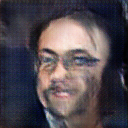
\includegraphics[width=120px]{./photos_from_epoch_8/samples_8_67.png}%
\caption{a man in a suit and tie holding a cell phone .}%
\end{figure}

%
\end{document}